\chapter{Shallow Water Solver}

\section{Synopsis}
The ShallowWaterSolver is a solver for depth-integrated wave 
equations of shallow water type. Presently the following equations 
are supported:

\begin{center}
\begin{tabular}{l|p{8cm}}
Value & Description \\
\hline
\inltt{LinearSWE} & Linearized SWE solver in primitive variables (constant
still water depth) \\
\inltt{NonlinearSWE} & Nonlinear SWE solver in conservative
variables (constant still water depth) \\
\hline
\end{tabular}
\end{center}

\subsection{The Shallow Water Equations}
The shallow water equations (SWE) is a two-dimensional system of nonlinear partial
differential equations of hyperbolic type that are fundamental in hydraulic, coastal
and environmental engineering. In deriving the SWE the vertical velocity is 
considered negligible and the horizontal velocities are assumed uniform with depth. 
The SWE are hence valid when the water depth can be considered small compared to the 
characteristic length scale of the problem, as typical for flows in rivers and shallow 
coastal areas. Despite the limiting restrictions the SWE can be used to describe many 
important phenomena, for example storm surges, tsunamis and river flooding. 

The two-dimensional SWE is stated in conservation form as
\begin{align*}
\frac{\partial {\mathbf U}}{\partial t} + \nabla \cdot {\mathbf F(U)} =
{\mathbf S(U)}\,
\end{align*}

where $\mathbf F(U) = \left[{\mathbf E(U)}\,, {\mathbf G(U)} \right]$ is the
flux vector and the vector of conserved variables read
${\mathbf U}=\left[H\,,Hu\,,Hv \right]^\mathrm{T}$. Here 
$H({\mathbf x},t)=\zeta({\mathbf x},t) + d({\mathbf x})$ is the total
water depth, $\zeta({\mathbf x},t)$ is the free surface elevation and
$d({\mathbf x})$ is the still water depth. The depth-averaged velocity
is denoted by ${\mathbf u}({\mathbf x},t) = \left[u,v\right]^\mathrm{T}$,
where $u$ and $v$ are the velocities in the $x$- and
$y$-directions, respectively. The content of the flux vector is
\begin{align*}
{\mathbf E(U)} = \left[ \begin{array}{c} Hu\\Hu^2 +
gH^2/2\\Huv\end{array}\right]\,, \qquad {\mathbf G(U)} = \left[
\begin{array}{c} Hv\\Hvu\\Hv^2 + gH^2/2\end{array}\right]\,,
\end{align*}

in which $g$ is the acceleration due to gravity. The source term
${\mathbf S(U)}$ accounts for, e.g., forcing due to bed
friction, bed slope, Coriolis force and higher-order dispersive effects 
(Boussinesq terms). In the distributed version of the ShallowWaterSolver
only the Coriolis force is included. 

\section{Usage}
\begin{lstlisting}[style=BashInputStyle]
ShallowWaterSolver session.xml
\end{lstlisting}

\section{Session file configuration}

\subsection{Solver Info}
\begin{itemize}
\item \inltt{Eqtype}: Specifies the equation to solve. This should be set
to \inltt{NonlinearSWE}.
\item \inltt{UpwindType}
\item \inltt{Projection}
\item \inltt{TimeIntegrationScheme}
\end{itemize}

\subsection{Parameters}
\begin{itemize}
\item \inltt{Gravity}
\end{itemize}

\subsection{Functions}
\begin{itemize}
\item \inltt{Coriolis}: Specifies the Coriolis force (variable name: `f`)
\item \inltt{WaterDepth}: Specifies the water depth (variable name: `d`)
\end{itemize}

\section{Examples}
\subsection{Rossby modon case}
This example, provided in \inltt{RossbyModon\_Nonlinear\_DG.xml} is of a
discontinuous Galerkin simulation of the westward propagation of an equatorial
Rossby modon.


\subsubsection{Input Options}

For what concern the ShallowWaterSolver the
\inltt{<SOLVERINFO>} section allows us to specify the solver, the type of
projection (continuous or discontinuous), the explicit time integration scheme to
use and (in the case the discontinuous Galerkin method is used) 
the choice of numerical flux. A typical example would be:
\begin{lstlisting}[style=XmlStyle]
 <SOLVERINFO>
   <I PROPERTY="EqType" VALUE="NonlinearSWE">
   <I PROPERTY="Projection" VALUE="DisContinuous">
   <I PROPERTY="TimeIntegrationMethod" VALUE="ClassicalRungeKutta4">
   <I PROPERTY="UpwindType" VALUE="HLLC">
 </SOLVERINFO>
\end{lstlisting}

In the \inltt{<PARAMETERS>} section we, in addition to the normal setting
of time step etc., also define the acceleration of gravity by 
setting the parameter "Gravity": 
\begin{lstlisting}[style=XmlStyle]
  <PARAMETERS>
     <P> TimeStep       = 0.04             </P>
     <P> NumSteps       = 1000             </P>
     <P> IO_CheckSteps  = 100              </P>
     <P> IO_InfoSteps   = 100              </P>
     <P> Gravity        = 1.0              </P>
  </PARAMETERS>
\end{lstlisting}

We specify $f$ which is the Coriolis parameter and $d$ denoting the
still water depth as analytic functions:
\begin{lstlisting}[style=XmlStyle]
<FUNCTION NAME="Coriolis">
    <E VAR="f" VALUE="0+1*y" />
</FUNCTION>

<FUNCTION NAME="WaterDepth">
    <E VAR="d" VALUE="1" />
</FUNCTION>
\end{lstlisting}

Initial values and boundary conditions are given in terms of primitive variables
(please note that also the output files are given in terms of primitive
variables). For the discontinuous Galerkin we typically enforce any slip wall boundaries
weakly using symmetry technique. This is given by the
\inltt{USERDEFINEDTYPE="Wall"} choice in the \inltt{<BOUNDARYCONDITIONS>}
section:
\begin{lstlisting}[style=XmlStyle]
  <BOUNDARYCONDITIONS>
    <REGION REF="0">
     <D VAR="eta"  USERDEFINEDTYPE="Wall"  VALUE="0" />
     <D VAR="u"    USERDEFINEDTYPE="Wall"  VALUE="0" />
     <D VAR="v"    USERDEFINEDTYPE="Wall"  VALUE="0" />
    </REGION>
  </BOUNDARYCONDITIONS>
\end{lstlisting}

\subsubsection{Running the code}

After the input file has been copied to the build directory
of the \inltt{ShallowWaterSolver} the code can be executed by:
\begin{lstlisting}[style=BashInputStyle]
 ./ShallowWaterSolver Rossby_Nonlinear_DG.xml
\end{lstlisting}

\subsubsection{Post-proceesing}
After the final time step the solver will write an output file 
\inltt{RossbyModon\_Nonlinear\_DG.fld}. We can convert it to tecplot
format by using the \inltt{FldToTecplot} utility. Thus we execute the
following command:
\begin{lstlisting}[style=BashInputStyle]
FldToTecplot RossbyModon_Nonlinear_DG.xml RossbyModon_Nonlinear_DG.fld 
\end{lstlisting}
This will generate a file called \inltt{RossbyModon\_Nonlinear\_DG.dat} that
can be loaded directly into tecplot:

\begin{figure}
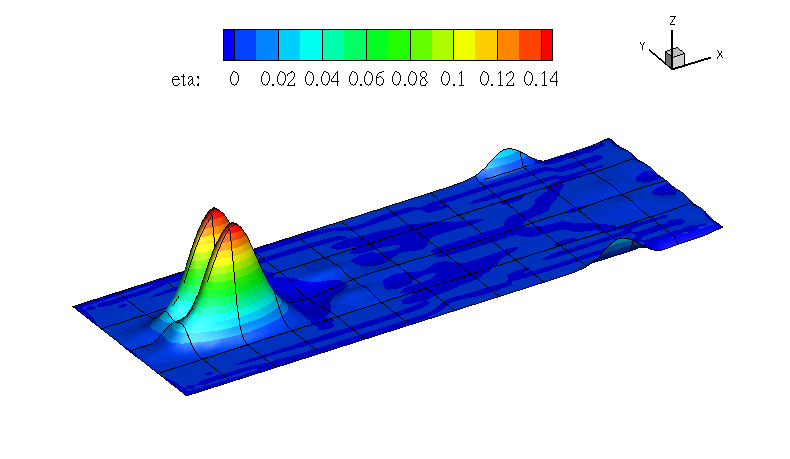
\includegraphics[width=\linewidth]{Figures/RossbyModon.png}
\end{figure}
